
The performance of the axiom weakening based repair algorithm shown in \cref{algo:repair-weaken} has also been evaluated. During each repair via axiom weakening, the required (real) time and the number of calls to the reasoner have been registered. Additionally, the number of steps taken by the repair using axiom weakening has been observed. Also, as mentioned in \cref{eval-quality}, the repair program was put under a timeout to prevent cases where the reasoning becomes unreasonably slow. The generation of inconsistent ontologies used a similar timeout, and the same procedure was used for situations in which the reasoner ran out of memory. The timeouts of the weakening procedure are shown separately from those latter cases in the results. The frequency of these cases is indicated as a percentage of the overall runs finished vs started. The results of this evaluation are presented in \cref{table:results-perf} and \cref{fig:results-perf-time}.

\begin{table}[ht]
  \scriptsize
  \centering
  \begin{tabular}{|l|r@{ }lr@{ }lr@{ }lr@{ }r|}
    \cline{2-9}
    \multicolumn{1}{l|}{} & \multicolumn{2}{c}{Steps} & \multicolumn{2}{c}{Calls} & \multicolumn{2}{c}{Time [ms]} & \multicolumn{2}{c|}{Failed} \\
    \hline
    admin & 6.3 & [4.0, 9.2] & 7621 & [5601, 10118] & 9638 & [5433, 14909] & 2\% & (2\%) \\
    ahso & 2.1 & [1.7, 2.5] & 4648 & [4228, 5131] & 11469 & [8122, 15336] & 11\% & (26\%) \\
    cdao & 2.1 & [1.8, 2.5] & 16137 & [14576, 17740] & 20767 & [15204, 27269] & 19\% & (48\%) \\
    cdpeo & 1.5 & [1.3, 1.7] & 4476 & [4250, 4716] & 2050 & [1942, 2169] & 0\% & (0\%) \\
    covid19-ibo & 1.3 & [1.2, 1.5] & 14822 & [14321, 15320] & 2208 & [2126, 2296] & 4\% & (13\%) \\
    ecp & 1.3 & [1.2, 1.5] & 2020 & [1916, 2133] & 4453 & [2738, 6939] & 1\% & (14\%) \\
    emo & 1.4 & [1.3, 1.6] & 18549 & [17473, 19615] & 6582 & [4439, 9688] & 1\% & (4\%) \\
    evi & 5.0 & [3.9, 6.4] & 5955 & [4680, 7425] & 4719 & [3408, 6349] & 19\% & (64\%) \\
    falls & 1.5 & [1.3, 1.6] & 1242 & [1161, 1331] & 874 & [843, 909] & 1\% & (5\%) \\
    fo & 1.6 & [1.4, 1.8] & 1295 & [1179, 1423] & 1090 & [1025, 1164] & 38\% & (61\%) \\
    gbm & 1.5 & [1.3, 1.6] & 7608 & [7070, 8131] & 2954 & [2808, 3117] & 0\% & (0\%) \\
    gfvo & 1.8 & [1.6, 2.0] & 4167 & [3864, 4501] & 2404 & [2258, 2569] & 0\% & (0\%) \\
    koro & 1.9 & [1.7, 2.2] & 6195 & [5697, 6706] & 2456 & [2277, 2648] & 0\% & (0\%) \\
    lico & 2.6 & [2.2, 2.9] & 6638 & [6105, 7186] & 3709 & [3400, 4077] & 1\% & (22\%) \\
    mamo & 2.5 & [2.2, 2.9] & 4667 & [4228, 5128] & 2215 & [2046, 2403] & 0\% & (0\%) \\
    mpio & 2.2 & [1.8, 2.6] & 1908 & [1720, 2133] & 987 & [913, 1078] & 9\% & (30\%) \\
    pizza & 2.0 & [1.7, 2.3] & 7550 & [6723, 8419] & 26767 & [20554, 34014] & 28\% & (55\%) \\
    provo & 4.9 & [3.7, 6.3] & 6851 & [5383, 8465] & 8878 & [5962, 12348] & 4\% & (8\%) \\
    qudt & 1.1 & [1.0, 1.2] & 7044 & [6816, 7291] & 6658 & [4229, 9672] & 9\% & (38\%) \\
    trans & 3.2 & [1.8, 5.1] & 4384 & [3213, 5894] & 3684 & [1610, 6513] & 0\% & (5\%) \\
    triage & 3.2 & [2.4, 4.3] & 5166 & [4255, 6351] & 8979 & [6084, 13102] & 28\% & (51\%) \\
    vio & 2.5 & [2.1, 3.0] & 9476 & [8628, 10327] & 15199 & [10496, 20803] & 3\% & (7\%) \\
    \hline
  \end{tabular}
  \caption{Results of the evaluation with respect to performance. The number of weakening iterations, reasoner calls, and total repair time are given as sample mean, with the 95\% confidence interval in brackets. The frequency of failed runs is shown as percentage of repairs by weakening that were started but not completed. In parentheses, the percentage of total failed runs, including those with timeout during generation of the inconsistent ontology. Attempts that failed were not considered for the other values.}
  \label{table:results-perf}
\end{table}

\begin{figure}[ht]
  \centering
  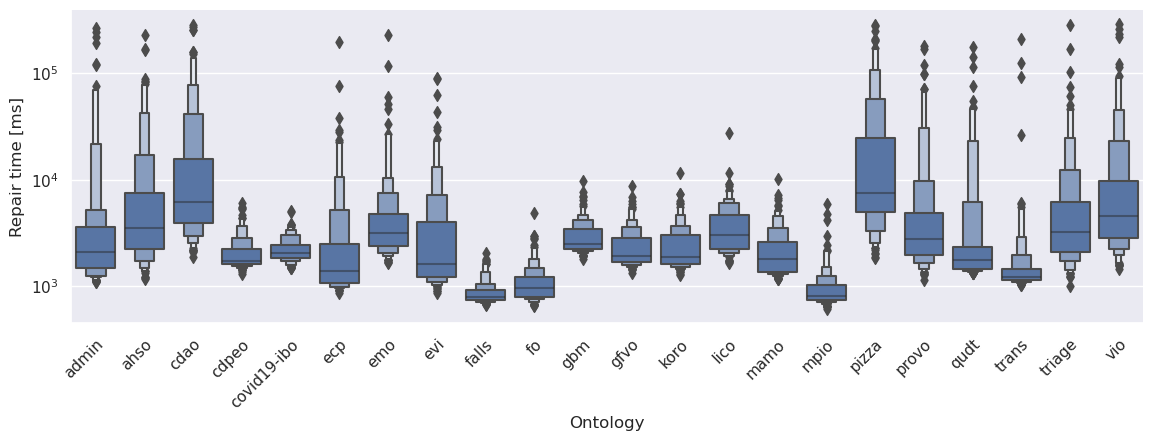
\includegraphics[width=\textwidth]{resources/time-ontology-violin.png}
  \caption{Distribution of (real) execution time required for repairing a single ontology using axiom weakening. The two darkest blue boxes represent (together) half of the samples, with the line in the middle indicating the median. Each lighter box represents half the samples of the boxes one step darker, and all remaining outliers are marked. Attempts that failed by a timeout or other errors were not considered.}
  \label{fig:results-perf-time}
\end{figure}

As is visible from the results, the number of reasoner calls and the execution time can vary significantly. The execution times were generally reasonable when a run was able to complete within the time limit, with most of them completing within 2 minutes, even though the time limit was set to 5 minutes. A significant number of runs, however, were affected by the timeout or other errors. It has not been looked deeper into what causes these issues.

